% !TeX encoding = UTF-8
\chapter{Task 3: Front-End Interface}\label{chap:task3}

The sample on the task sheet shows a dark page with a dropdown of local interfaces, a timespan field, a \emph{Start Packet Capture} button and a table called \emph{Algorithm Output} with source and destination address and port, a timestamp and the result (Normal or Malicious). We built the same page (\texttt{web/index.html}, one file with HTML, CSS and JavaScript, no external libraries) and a small server (\texttt{script/webui.py}, Python standard library only) that uses the same \texttt{Session} class as the command-line agent.

\section{Controls and API}
\begin{itemize}\setlength\itemsep{0pt}
	\item \textbf{Available Local Interfaces:} filled from \texttt{GET /api/interfaces}. The management interface \texttt{mgmt0} is hidden, so the page cannot attach a program to the interface that carries its own traffic. The default is \texttt{ext0}.
	\item \textbf{Enter Timespan:} seconds, 1 to 3600.
	\item \textbf{Model:} DT, XGB or ALL (we added this dropdown to the sample).
	\item \textbf{Replay dataset flows:} number of test-split flows replayed through the kernel program at random times over the first 80\,\% of the capture, interleaved with live flows (default 20, 0 to 100; Section~\ref{sec:replay}).
	\item \textbf{Start Packet Capture / Stop:} \texttt{POST /api/start} answers 202, 400 for invalid input or 409 if a capture is already running on the interface; \texttt{POST /api/stop} ends it.
	\item \textbf{Status line and table:} the page polls \texttt{GET /api/flows}. The status line shows the remaining time and the counters (packets, dropped, classified, malicious, blocks). Malicious rows are red. The Models column shows the verdict of each model.
\end{itemize}
The server validates every field (interface, timespan, model, a request body of at most 4\,KB). It listens only on the management address 172.28.0.2:8080, so the browser on the host can reach it, but the client behind the XDP hook cannot, and its own polling never crosses \texttt{ext0}.

\section{Screenshots}
Each capture replays 20 dataset flows (half benign, half DDoS), so the table holds at least 20 rows with a random mix of Normal and Malicious, together with the live client flows (172.28.1.20). Figure~\ref{fig:SS_T3_3} shows the ALL capture: the status line reads 335 packets, 8 dropped, 55 classified, 7 malicious and 7 blocks. The DT and XGB captures look the same and were also run. The blocked sources are replayed 10.99.x.y addresses, and the client 172.28.1.20 stays Normal.

\begin{figure}[H]
	\centering
	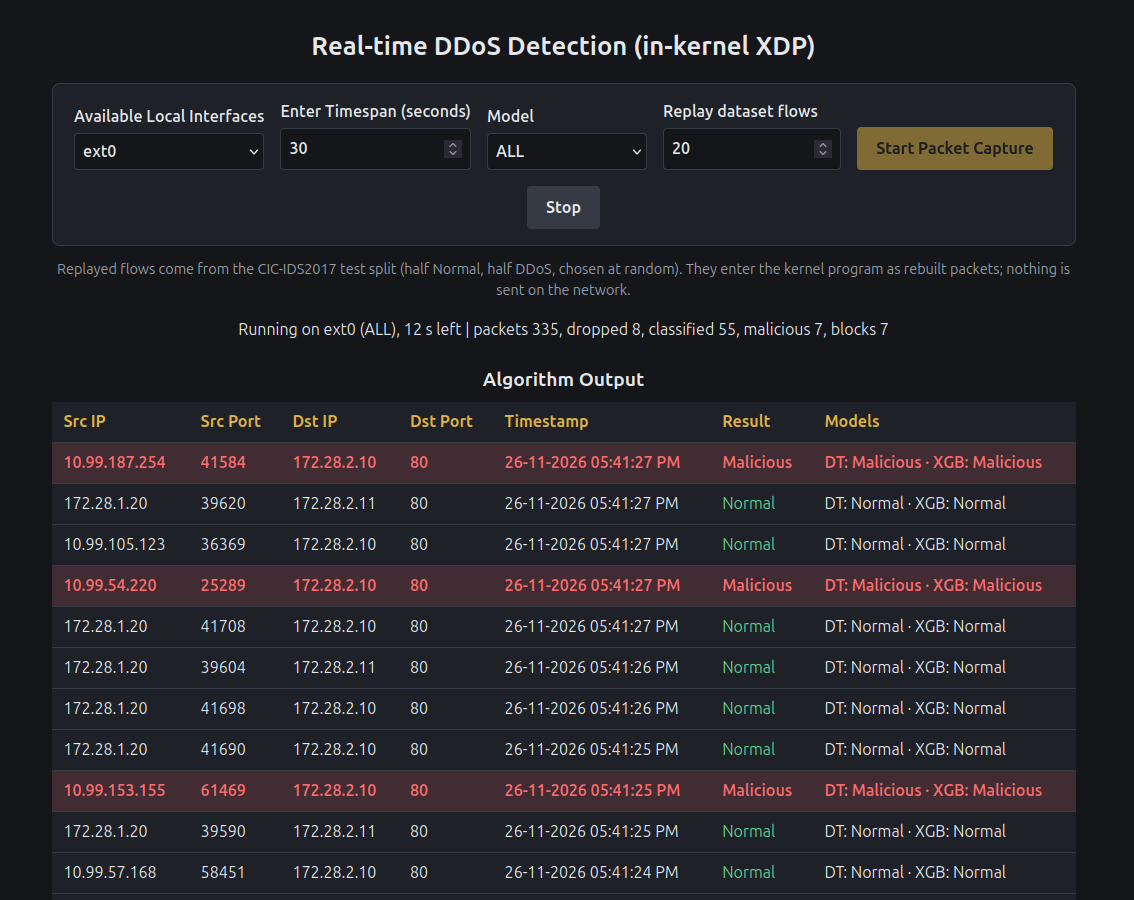
\includegraphics[width=0.85\linewidth,height=0.38\textheight,keepaspectratio]{../SS/SS_T3_3.png}
	\caption{Web interface with both models (\texttt{ALL}): Malicious rows need both verdicts.}\label{fig:SS_T3_3}
\end{figure}
